\documentclass[10pt]{article}
\usepackage[utf8]{inputenc}
\usepackage[activeacute,spanish]{babel}
\usepackage[left=1.5cm,top=1.5cm,right=1.5cm, bottom=1.5cm,letterpaper, includeheadfoot]{geometry}

\usepackage{amssymb, amsmath, amsthm}
\usepackage{graphicx}
\usepackage{hyperref}
\usepackage{lmodern,url}
\usepackage{paralist} %util para listas compactas
\usepackage{xcolor}
\usepackage{bbm}
\usepackage{mathrsfs}
\usepackage{bbm}

%========PAQUETES AGREGADOS===========
%Pseudocodigo
\usepackage{pseudocode}
\usepackage[portuguese, boxruled]{algorithm2e}
\usepackage{wrapfig}
\usepackage{multicol}
\usepackage{graphicx}
\usepackage{caption}
\usepackage{subcaption}
%\captionsetup[table]{labelformat=empty}
\captionsetup[subfigure]{labelformat=empty}
\usepackage{cancel}
%====================================

\usepackage{fancyhdr}
\pagestyle{fancy}
\fancypagestyle{plain}{%
\fancyhf{}
\lhead{\footnotesize\itshape\bfseries\rightmark}
\rhead{\footnotesize\itshape\bfseries\leftmark}
}


% macros
\newcommand{\Q}{\mathbb Q}
\newcommand{\R}{\mathbb R}
\newcommand{\N}{\mathbb N}
\newcommand{\Z}{\mathbb Z}
\newcommand{\C}{\mathbb C}
\newcommand{\BigO}{\mathcal{O}}
%Teoremas, Lemas, etc.
\theoremstyle{plain}
\newtheorem{teo}{Teorema}
\newtheorem{lem}{Lema}
\newtheorem{prop}{Proposición}
\newtheorem{cor}{Corolario}
\newtheorem{obs}{Observación}
\newtheorem{ej}{Ejemplo}
\renewcommand{\qedsymbol}{\rule{0.7em}{0.7em}}
\renewenvironment{proof}{{\bfseries \noindent Demostración}}{ \qed \\}


\theoremstyle{definition}
\newtheorem{defi}{Definición}
% fin macros


\newcommand{\catnum}{6} %numero de catedra
\newcommand{\fecha}{13 de Septiembre 2016 }

%%%%%%%%%%%%%%%%%%

%Macros para este documento
\newcommand{\cin}{\operatorname{cint}}



\begin{document}
%Encabezado
\fancyhead[L]{Facultad de Ciencias Físicas y Matemáticas}
\fancyhead[R]{Universidad de Chile}
\vspace*{-1.2 cm}
\begin{minipage}{0.6\textwidth}
\begin{flushleft}
\hspace*{-0.5cm}\textbf{MA3402-1 Estadística. Primavera 2016}\\
\hspace*{-0.5cm}\textbf{Profesor:} Raul Gouet\\
\hspace*{-0.5cm}\textbf{Escriba:} Manuel Cáceres\\
\hspace*{-0.5cm}\textbf{Fecha:} \fecha
\end{flushleft}
\end{minipage}
\begin{minipage}{0.36\textwidth}
\begin{flushright}

\includegraphics[scale=0.3]{imagenes/fcfm_dcc}
\end{flushright}
\end{minipage}
\bigskip
%Fin encabezado

\begin{center}
\LARGE\textbf{Clase \catnum}
\end{center}
Recordemos la estimación de máxima verosimilitud (Fischer).\\
$X$ con función de densidad $f_{\theta}(x), \theta \in \Theta$, $L(\theta) = f_{\theta}(x)$ (verosimilitud de x), $\hat{\theta}(X) \in arg\max_{\theta \in \Theta} L(\theta)$ (Estimador de máxima verosimilitud (EMV))
\begin{ej} Modelo Gaussiano, $(X_{1},X_{2},\ldots,X_{n})$ v.a. iid $\mathcal{N}(\mu, \sigma^2)$\\
$X = (X_{1},X_{2},\ldots,X_{n}), \theta = (\mu, \sigma) \in \Theta = \mathbb{R}\times (0,\infty)$
\begin{align*}
f_{\theta}(x) &= \left(\frac{1}{\sqrt{2\pi}\sigma}\right)^n e^{\frac{1}{2}\sum\left(\frac{x_{i}-\mu}{\sigma}\right)^2}\\
l(\theta) &= \log L(\theta) = k - n\log \sigma - \frac{1}{2\sigma^2}\sum\left(x_{i}-\mu\right)^2\\
\frac{\partial l}{\partial \mu} &= \frac{2}{2\sigma^2}\sum (x_{i}-\mu) = 0 \Leftrightarrow \hat{\mu} = \frac{1}{n}\sum x_{i} = \bar{X}, \forall \sigma
\end{align*}
Por lo que $\hat{\mu}(X) = \bar{X}$ es el EMV de $\mu$.\\
Buscamos ahora el maximizante respecto a $\sigma$.\\
Aprovechamos que $\hat{\mu}$ es maximizante para estudiar $l(\bar{X},\sigma)$ en lugar de $l(\mu, \sigma)$.\\
\begin{eqnarray*}
& l(\bar{X}, \sigma) & = k - n\log \sigma - \frac{1}{2\sigma^2}\sum(X_{i}-\bar{X})^2\\
& \frac{\partial l}{\partial \sigma} & = -\frac{n}{\sigma} + \frac{1}{\sigma^3}\sum (X_{i}-\bar{X})^2 = 0\\
\Rightarrow & \hat{\sigma}^2 & = \frac{1}{n}\sum (X_{i}-\hat{X})^2
\end{eqnarray*}
Diríamos que $\hat{\sigma}(x) = \sqrt{\frac{1}{n}\sum (x_{i}-\hat{x})^2}$ es el EMV de $\sigma$ (hay que comprobar que tenemos un max).\\
Como definición, el EMV de $g(\theta)$ es $g(\hat{\theta})$, donde $\hat{\theta}$ es EMV de $\theta$.\\
Por lo tanto, $\hat{\sigma}^2 = \frac{1}{n}\sum(x_{i}-\bar{x})^2$ es EMV de la $\sigma^2$ (la varianza de la normal)
\end{ej}
\begin{obs}Se tiene que:\\
\begin{itemize}
\item $\hat{\mu}(x)$ es insesgado para $\mu$
\item $\hat{\sigma}^2$ NO es insesgado para $\sigma^2$
\item $\hat{\sigma}$ NO es insesgado para $\sigma$
\end{itemize}
\end{obs}
Es sencillo calcular
\begin{align*}
\mathbb{E}_{\theta}(\hat{\sigma}^2(x)) &= \mathbb{E}_{\theta}(\frac{1}{n}\sum (x_{i}-\bar{x})^2)\\
&= \frac{1}{n}\sum \mathbb{E}_{\theta} (x_{i}-\bar{x})^2
\end{align*}

Se calcula $\mathbb{E}_{\theta}\left((x_{i}-\bar{x})^2\right)$, sumando y restando $\mu$ o bien volviendo a la expresión para la media y desarrollando.
\begin{align*}
\mathbb{E}_{\theta}\left(x_{i}-\bar{x}\right)^2 &= \mathbb{E}_{\theta}\left((x_{i}-\mu - (\bar{x}-\mu))^2\right)\\
&= \mathbb{E}_{\theta}\left((x_{i}-\mu)^2\right) + \mathbb{E}_{\theta}\left((\bar{x}-\mu^2)\right) - 2\mathbb{E}_{\theta}((x_{i}-\mu)(\bar{x}-\mu))\\
&= \sigma^2 + \frac{\sigma^2}{n} - 2 Cov_{\theta}(x_{i},\bar{x})\\
&= \frac{1}{n} Cov_{\theta}(x_{i},\sum x_{j})\\
&= \frac{1}{n} \sum_{j} Cov_{\theta}(x_{i},x_{j})\\
&= \frac{1}{n} \frac{Cov_{\theta}(x_{i},x_{j})}{\sigma^2}
\end{align*}
Resulta entonces que $S^2 = \frac{1}{n-1}\sum (x_{i}-\bar{x})^2$ es insesgado para $\sigma^2$ pero no es EMV.\\
Sin embargo, $\sqrt{S^2}$ no es insesgado para $\sigma$.

\begin{ej} Caso uniforme\\
Sea $X_{1},\ldots,X_{n}$ iid uniforme $\left[0,\theta\right], \theta > 0$.\\
\begin{align*}
f_{\theta}(x) = \prod \mathbbm{1}_{(0,\theta)}(x_{i})\frac{1}{\theta} = \frac{1}{\theta^n}\mathbbm{1}_{\{0 \le min\ x \le max\ x \le \theta\}}\\
\max_{\theta > 0} L(\theta) = \max_{\theta > 0} \frac{1}{\theta^n}\mathbbm{1}_{\{0 \le y(x) =  min\ x \le max\ x = z(x) \le \theta\}}
\end{align*}
Graficando obtenemos :\\
\begin{center}
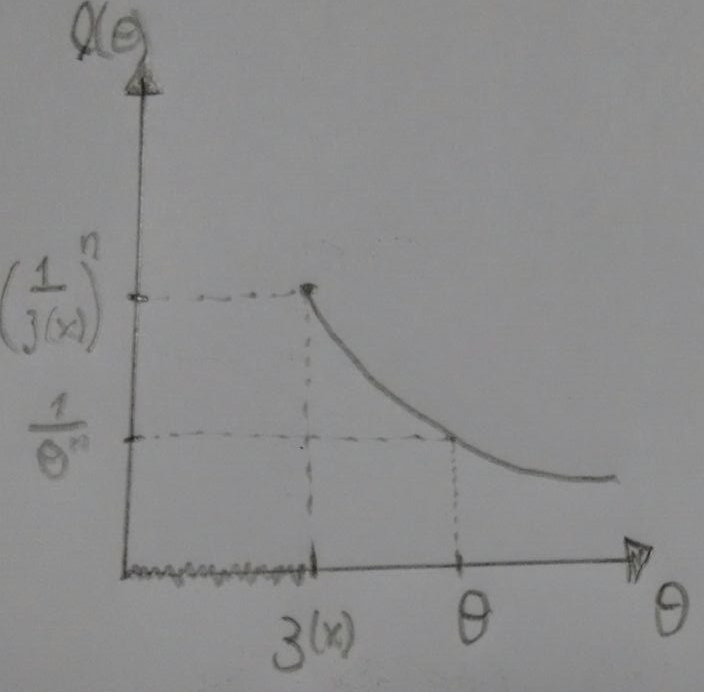
\includegraphics[scale=0.2]{imagenes/emv_uniforme.png}
\end{center}
El máximo se alcanza en $\hat{\theta}(x) = z(x)$. Notar que $\mathbb{E}(\hat{\theta}(x)) < \theta$, por lo que el EMV no es insesgado, pero puede corregirse este sesgo.
\end{ej}
\begin{ej} Segundo caso uniforme\\
$X_{1},\ldots,X_{n}$ iid $\mathcal{U}[\theta, \theta +1], \theta > 0$\\
\begin{align*}
f_{\theta}(x) &= \prod \mathbbm{1}_{[\theta,\theta+1]}(x_{i})\\
&= \mathbbm{1}_{\{\theta \le y(x) \le z(x) \le \theta+1\}}
\end{align*}
Es decir, cualquier $\hat{\theta}(x)$ que satisfasga $z(x)-1 \le \theta \le y(x)$ es EMV, por ejemplo:
\begin{itemize}
\item $\hat{\theta}(x) = y(x)$
\item $\hat{\theta}(x) = z(x)-1$
\item $\hat{\theta}(x) = \frac{y(x)+z(x)-1}{2}$
\end{itemize}
En realidad sirve cualquier combinación convexa de los extremos, pero, por ejemplo, no sirve la media de las estimaciones.
\end{ej}

\begin{ej} Cadena con 2 estados\\
\begin{center}
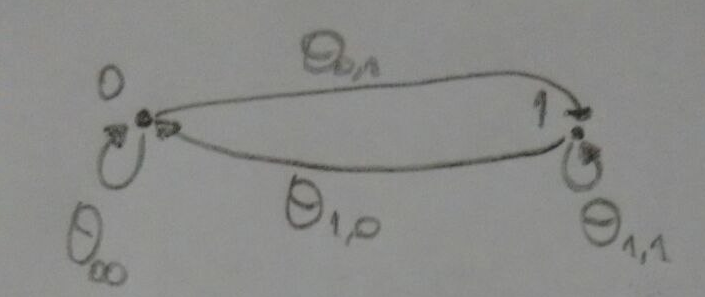
\includegraphics[scale=0.2]{imagenes/cadena.png}
\end{center}
Podemos definir la sucesión de variables aleatorias $(X_{n})_{n\ge 0}$ (o cadena de Markov) como el estado en el que se encuentra el autómata en el paso $n$(para cada $n$) (la probabilidad viene dada por los $\theta s$ que representan la probabilidad de seguir esa transición). Notemos que estas variables aleatorias son dependientes (pues las probabilidades del siguiente estado dependen del estado en el que estoy), pero no guardan historia, es decir, una variable aleatoria solo depende de la anterior (propiedad markoviana). Con esto podemos definir la densidad como :
\begin{align*}
\mathbb{P}_{\theta}(X_{1}=x_{1},\ldots,X_{n}=x_{n}) &= \mathbb{P}_{\theta}(X_{0}=x_{0})\mathbb{P}_{\theta}(X_{1}=x_{1}|X_{0}=x_{0})\ldots \mathbb{P}_{\theta}(X_{n}=x_{n}|X_{n-1}=x_{n-1})
\end{align*}
Ahora bien
\begin{align*}
\forall i \ge 1, \mathbb{P}_{\theta}(X_{i}=x_{i}|X_{i-1}=x_{i-1}) = \left\{
\begin{array}{c l}
 \theta_{00} & X_{i-1}=X_{i}=0\\
 \theta_{01} & X_{i-1}=0, X_{i}=1\\
 \theta_{10} & X_{i-1}=1, X_{i}=0\\
 \theta_{11} & X_{i-1}=X_{i}=1
\end{array}
\right.
\end{align*}
Y se tienen las restricciones
\begin{align*}
\theta_{00} + \theta_{01} = 1\\
\theta_{10} + \theta_{11} = 1
\end{align*}
Así llegamos a 
\begin{align*}
f_{\theta} = \lambda(x_{0}) \theta_{00}^{\sum (1-x_{i})(1-x_{i-1})} \theta_{01}^{\sum (1-x_{i-1})x_{i}}\theta_{10}^{\sum x_{i-1}(1-x_{i})} \theta_{11}^{\sum x_{i}x_{i-1}}
\end{align*}
Maximizando esto en $\theta_{00}$ llegamos a que
\begin{align*}
\hat{\theta}_{00} = \frac{\frac{\sum (1-x_{i-1})(1-x_{i})}{\sum (1-x_{i-1})(1-x_{i}) + \sum (1-x_{i-1})x_{i}}}{\sum (1-x_{i-1})}
\end{align*}
\end{ej}
\section{Estimación por conjuntos (de confianza)}
Buscamos un conjunto (o intervalo en caso real) que contenga ``plausiblemente'' los valores de una función $g(\theta)$ del parámetro desconocido $\theta$.\\
Este conjunto debería depender de nuestros datos obviamente y debería ser razonablemente pequeño (útil).\\
¿De dónde sacar este conjunto?\\
Supongamos que se estima $g(\theta)$ a valores en $\mathbb{R}$ con el estimador $\hat{g}(X)$ insesgado.\\
Se sabe que $\mathbb{V}_{\theta}(\hat{g}(X)) = \sigma^2(\theta)$, la cual somos capaces de estimar con $\hat{\sigma}^2(X)$.\\
Proclamamos el intervalo $[\hat{g}(X)- \sqrt{\hat{\sigma}^2(X)}, \hat{g}(X)+ \sqrt{\hat{\sigma}^2(X)}]$
\end{document}